\documentclass[10pt]{article}

\textwidth 16cm \textheight 23cm \evensidemargin 0cm
\oddsidemargin 0cm \topmargin -2cm
\parindent 0pt
\parskip \medskipamount


\usepackage[dutch]{babel}
\usepackage{amssymb}
\usepackage{amsmath}
\usepackage[utf8]{inputenc}
\usepackage[normalem]{ulem} % strikethrough normal text with \sout{text}
\usepackage{cancel} % strikethrough in math mode with \cancel{text}
\usepackage{graphicx}
\usepackage{pgf,tikz}
\usetikzlibrary{arrows}

\title{Bouwplannen Perfecte Vierkanten}
\author{Pieter Pareit}

\usepackage[pdfauthor=Pieter Pareit,pdftitle=Bouwplannen Perfecte Vierkanten]{hyperref}

\begin{document}

\section*{Bouwplannen Perfecte Vierkanten}

\subsection*{Perfecte vierkanten}

Een {\bf perfect vierkant} van orde $n$ is een vierkant dat opgedeeld is in $n$ verschillende vierkanten waarvan geen twee vierkanten even groot zijn.

Het eerste perfecte vierkant werd in $1939$ gevonden door Roland Sprague. Dit perfecte vierkant had orde $55$. In de jaren daarop vond men nog meer perfecte vierkanten, ook van kleinere orde. In $1962$ begon de Nederlandse informaticus Adrianus Duijvestijn een zoektocht naar het perfecte vierkant met de laagste orde. Het duurde nog tot $1978$ voordat computers snel en krachtig genoeg waren om dit probleem op te lossen. Het perfecte vierkant met de laagste orde wordt opgebouwd met $21$ kleinere vierkantjes en staat afgebeeld in Figuur \ref{fig:pv21}.

\begin{figure}[ht]
  \centering
  {\small
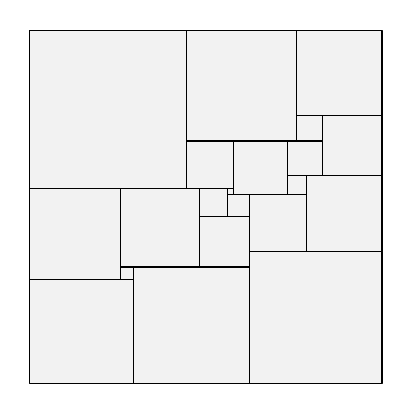
\begin{tikzpicture}[scale=0.04,line cap=round,line join=round,>=triangle 45,x=1.0cm,y=1.0cm]
\clip(-0.5,-0.5) rectangle (113,113);
\filldraw[fill=black,fill opacity=0.05] (0,0) -- (33,0) -- (33,33) -- (0,33) -- cycle;
\filldraw[fill=black,fill opacity=0.05] (33,0) -- (70,0) -- (70,37) -- (33,37) -- cycle;
\filldraw[fill=black,fill opacity=0.05] (70,0) -- (112,0) -- (112,42) -- (70,42) -- cycle;
\filldraw[fill=black,fill opacity=0.05] (0,33) -- (29,33) -- (29,62) -- (0,62) -- cycle;
\filldraw[fill=black,fill opacity=0.05] (29,33) -- (33,33) -- (33,37) -- (29,37) -- cycle;
\filldraw[fill=black,fill opacity=0.05] (0,62) -- (50,62) -- (50,112) -- (0,112) -- cycle;
\filldraw[fill=black,fill opacity=0.05] (29,62) -- (29,37) -- (54,37) -- (54,62) -- cycle;
\filldraw[fill=black,fill opacity=0.05] (54,37) -- (70,37) -- (70,53) -- (54,53) -- cycle;
\filldraw[fill=black,fill opacity=0.05] (70,42) -- (88,42) -- (88,60) -- (70,60) -- cycle;
\filldraw[fill=black,fill opacity=0.05] (88,42) -- (112,42) -- (112,66) -- (88,66) -- cycle;
\filldraw[fill=black,fill opacity=0.05] (54,53) -- (63,53) -- (63,62) -- (54,62) -- cycle;
\filldraw[fill=black,fill opacity=0.05] (63,53) -- (70,53) -- (70,60) -- (63,60) -- cycle;
\filldraw[fill=black,fill opacity=0.05] (63,60) -- (65,60) -- (65,62) -- (63,62) -- cycle;
\filldraw[fill=black,fill opacity=0.05] (82,60) -- (88,60) -- (88,66) -- (82,66) -- cycle;
\filldraw[fill=black,fill opacity=0.05] (65,60) -- (82,60) -- (82,77) -- (65,77) -- cycle;
\filldraw[fill=black,fill opacity=0.05] (50,62) -- (65,62) -- (65,77) -- (50,77) -- cycle;
\filldraw[fill=black,fill opacity=0.05] (50,112) -- (50,77) -- (85,77) -- (85,112) -- cycle;
\filldraw[fill=black,fill opacity=0.05] (82,77) -- (82,66) -- (93,66) -- (93,77) -- cycle;
\filldraw[fill=black,fill opacity=0.05] (93,66) -- (112,66) -- (112,85) -- (93,85) -- cycle;
\filldraw[fill=black,fill opacity=0.05] (85,77) -- (93,77) -- (93,85) -- (85,85) -- cycle;
\filldraw[fill=black,fill opacity=0.05] (85,85) -- (112,85) -- (112,112) -- (85,112) -- cycle;
\end{tikzpicture}
}

  \caption{Perfect vierkant van orde $21$.}
  \label{fig:pv21}
\end{figure}

\subsection*{Zelf een perfect vierkant bouwen}

We kunnen een perfect vierkant construeren met vierkante stukjes karton. Als we als éénheden centimeter nemen, dan heeft het perfecte vierkant van orde $21$ zijden van $112$ cm. Dit is te groot, laten we daarom alles herschalen met factor $\frac{1}{4}$. De zijden zullen dan $28$ cm zijn. Om het perfecte vierkant van orde $21$ te bouwen hebben we dan de vierkante stukjes karton nodig uit Tabel \ref{tbl:bouwplan:21}.

\begin{table}[ht]
  \centering
  \begin{tabular}{c|c||c|c||c|c}
    grootte & uit te knippen & grootte & uit te knippen & grootte & uit te knippen\\
    \hline
    $2\times 2$ & $0,5$ cm op $0,5$ cm & $15\times 15$ & $3,75$ cm op $3,75$ cm & $27\times 27$ & $6,75$ cm op $6,75$ cm\\
    $4\times 4$ & $1$ cm op $1$ cm & $16\times 16$ & $4$ cm op $4$ cm & $29\times 29$ & $7,25$ cm op $7,25$ cm\\
    $6\times 6$ & $1,5$ cm op $1,5$ cm & $17\times 17$ & $4,25$ cm op $4,25$ cm & $33\times 33$ & $8,25$ cm op $8,25$ cm\\
    $7\times 7$ & $1,75$ cm op $1,75$ cm & $18\times 18$ & $4,5$ cm op $4,5$ cm & $35\times 35$ & $8,75$ cm op $8,75$ cm\\
    $8\times 8$ & $2$ cm op $2$ cm & $19\times 19$ & $4,75$ cm op $7,75$ cm & $37\times 37$ & $9,25$ cm op $9,25$ cm\\
    $9\times 9$ & $2,25$ cm op $2,25$ cm & $24\times 24$ & $6$ cm op $6$ cm & $42\times 42$ & $10,5$ cm op $10,5$ cm\\
    $11\times 11$ & $2,75$ cm op $2,75$ cm & $25\times 25$ & $6,25$ cm op $6,25$ cm & $50\times 50$ & $12,5$ cm op $12,5$ cm\\
  \end{tabular}
  \caption{Bouwplan voor het perfecte vierkant van orde $21$.}
  \label{tbl:bouwplan:21}
\end{table}

Omdat er aan bovenstaand perfect vierkant nog weinig uitdagend puzzelwerk is, staan in Tabel \ref{tbl:bouwplan:22} de benodigdheden om $8$ perfecte vierkanten te construeren van orde $22$. Spreek af met je collega-studenten welke kolom van vierkanten jij zult uitknippen en wissel dan de puzzels uit. Markeer op elk stukje ook welke grootte het heeft (niet de herschaalde grootte) en tot welke puzzel het behoord (van 1 tot 8).

\begin{table}[ht]
  \centering
  \begin{tabular}{c|c||c|c||c|c||c|c||c|c||c|c||c|c||c|c}
  gr & $\frac{1}{4}\cdot$gr & gr & $\frac{1}{4}\cdot$gr & gr & $\frac{1}{4}\cdot$gr & gr & $\frac{1}{4}\cdot$gr & gr & $\frac{1}{4}\cdot$gr & gr & $\frac{1}{4}\cdot$gr & gr & $\frac{1}{4}\cdot$gr & gr & $\frac{1}{4}\cdot$gr\\
  \hline
  2 & 0.5   & 1 & 0.25  & 1 & 0.25   & 1 & 0.25   & 2 & 0.5    & 2 & 0.5    & 1 & 0.25   & 4 & 1  \\
  3 & 0.75  & 2 & 0.5   & 2 & 0.5    & 3 & 0.75   & 4 & 1      & 5 & 1.25   & 2 & 0.5    & 8 & 2  \\
  4 & 1     & 3 & 0.75  & 3 & 0.75   & 4 & 1      & 8 & 2      & 9 & 2.25   & 3 & 0.75   & 9 & 2.25  \\
  6 & 1.5   & 4 & 1     & 4 & 1      & 5 & 1.25   & 10 & 2.5   & 11 & 2.75  & 4 & 1      & 10 & 2.5  \\
  7 & 1.75  & 6 & 1.5   & 7 & 1.75   & 8 & 2      & 11 & 2.75  & 16 & 4     & 9 & 2.25   & 12 & 3  \\
  8 & 2     & 8 & 2     & 8 & 2      & 9 & 2.75   & 12 & 3     & 17 & 4.25  & 11 & 2.75  & 14 & 3.5  \\
  12 & 3    & 9 & 2.25  & 10 & 2.5   & 17 & 4.25  & 15 & 3.75  & 19 & 4.75  & 13 & 3.25  & 17 & 4.25   \\
  13 & 3.25 & 12 & 3    & 17 & 4.25  & 20 & 5     & 19 & 4.75  & 21 & 5.25  & 16 & 4     & 19 & 4.75  \\
  14 & 3.5  & 14 & 3.5  & 18 & 4.5   & 21 & 5.25  & 21 & 5.25  & 22 & 5.5   & 17 & 4.25  & 26 & 6.5  \\
  15 & 3.75 & 16 & 4    & 20 & 5     & 23 & 5.75  & 22 & 5.5   & 24 & 6     & 18 & 4.5   & 28 & 7  \\
  16 & 4    & 17 & 4.25 & 21 & 5.25  & 25 & 6.25  & 23 & 5.75  & 26 & 6.5   & 19 & 4.75  & 31 & 7.75  \\
  17 & 4.25 & 18 & 4.5  & 22 & 5.75  & 26 & 6.5   & 25 & 6.25  & 30 & 7.5   & 22 & 5.5   & 35 & 8.75  \\
  18 & 4.5  & 19 & 4.75 & 24 & 6     & 29 & 7.25  & 26 & 6.5   & 31 & 7.75  & 24 & 6     & 36 & 9  \\
  21 & 5.25 & 21 & 5.25 & 27 & 6.75  & 31 & 7.75  & 32 & 8     & 33 & 8.25  & 33 & 8.25  & 37 & 9.25  \\
  22 & 5.5  & 22 & 5.5  & 28 & 7     & 32 & 8     & 34 & 8.5   & 35 & 8.75  & 36 & 9     & 41 & 10.25  \\
  23 & 5.75 & 23 & 5.75 & 29 & 7.25  & 40 & 10    & 37 & 9.25  & 36 & 9     & 38 & 9.5   & 47 & 11.75  \\
  24 & 6    & 24 & 6    & 30 & 7.5   & 43 & 10.75 & 41 & 10.25 & 41 & 10.25 & 39 & 9.75  & 49 & 12.25     \\
  26 & 6.5  & 26 & 6.5  & 31 & 7.75  & 44 & 11    & 43 & 10.75 & 46 & 11.5  & 42 & 10.5  & 57 & 14.25    \\
  27 & 6.75 & 27 & 6.75 & 32 & 8     & 47 & 11.75 & 45 & 11.25 & 47 & 11.75 & 44 & 11    & 59 & 14.75   \\
  28 & 7    & 28 & 7    & 38 & 9.5   & 48 & 12    & 47 & 11.75 & 50 & 12.5  & 53 & 13.25 & 62 & 15.5     \\
  50 & 12.5 & 50 & 12.5 & 59 & 14.75 & 52 & 13    & 55 & 13.75 & 52 & 13    & 75 & 18.75 & 71 & 17.75   \\
  60 & 15   & 60 & 15   & 80 & 20    & 55 & 13.75 & 59 & 14.75 & 61 & 15.25 & 97 & 24.25 & 86 & 21.5      \\
  \end{tabular}
  \caption{De 8 bouwplannen voor alle perfecte vierkanten van orde 22.}
  \label{tbl:bouwplan:22}
\end{table}

Het construeren van een perfect vierkant is een ganse uitdaging. Zonder hulp van computers is het bijna onmogelijk om alle perfecte vierkanten te vinden van een gegeven orde. Het in elkaar puzzelen van een perfect vierkant als je alle vierkanten krijgt waaruit het opgebouwd is wel haalbaar. Veel puzzelplezier!

\subsection*{De oplossingen}

We geven nu nog de oplossingen van de acht perfecte vierkanten van orde $22$. Om niet elk perfect vierkant te moeten tekenen maken we gebruik van een eenvoudige notatie (deze staat in de literatuur bekend als de Bouwkamp code). In deze notatie gebruiken we rechthoekige haakjes om naast elkaar liggende vierkanten, waarbij de bovenkanten van de vierkanten steeds op dezelfde hoogte liggen, te groeperen. De groepjes worden dan sequentieel geplaatst in de hoogste en meest linkse positie. Zo is de Bouwkamp code van het perfecte vierkant van orde $21$ uit Figuur \ref{fig:pv21} gegeven door:
$$
[50, 35, 27], [8, 19], [15, 17, 11], [6, 24], [29, 25, 9, 2], [7, 18], [16], [42], [4, 37], [33].
$$

De Bouwkamp codes voor de 8 perfecte vierkanten van orde $22$ zijn
\begin{enumerate}
  \item $[60,50], [23,27], [24,22,14], [7,16], [8,6], [12,15], [13], [2,28], [26], [4,21,3], [18], [17]$;
  \item $[60,50], [27,23], [24,22,14], [4,19], [8,6], [3,12,16], [9]], [2,28], [26], [21], [1,18], [17]$;
  \item $[80,59], [21,38], [29,28,17,27], [7,10], [18,20], [4,3], [32,8], [1,31], [30], [24,2], [22]$;
  \item $[55,44,48], [40,4], [52], [26,29], [23,3], [20,31,21], [5,47], [43], [9,17], [1,8], [32], [25]$;
  \item $[59,43,45], [41,2], [47], [34,25], [21,37,8], [55], [22,12], [10,23], [32], [11,26], [19,4], [15]$;
  \item $[61,52,41], [11,30], [9,35,19], [46,24], [16,33], [22,2], [36,17], [50], [47,21], [5,31], [26]$;
  \item $[97,75], [22,53], [39,42,38], [9,44], [4,19,13,2], [36,3], [11], [33,16], [24], [1,18], [17]$;
  \item $[86,49,57], [41,8], [28,37], [19,9], [47,35,4], [31,14], [10,36], [17,26], [12,71], [62], [59]$.
\end{enumerate}

\end{document}























